%%%%%%%% MLSys 2024 FINAL REPORT %%%%%%%%%%%%%%%%%

\documentclass{article}

\begin{filecontents*}{references.bib}
@article{jin2025ragcache,
  author    = {Jin, Chao and Zhang, Zili and Jiang, Xuanlin and Liu, Fangyue and Liu, Xin and Liu, Xuanzhe and Jin, Xin},
  title     = {{RAGCache}: Efficient Knowledge Caching for Retrieval-Augmented Generation},
  journal   = {ACM Transactions on Computer Systems},
  year      = {2025},
  volume    = {44},
  number    = {1},
  pages     = {1--27},
  publisher = {Association for Computing Machinery},
  doi       = {10.1145/3768628}
}

@inproceedings{yao2025cacheblend,
  author    = {Yao, Jiayi and Li, Hanchen and Liu, Yuhan and Ray, Siddhant and Cheng, Yihua and Zhang, Qizheng and Du, Kuntai and Lu, Shan and Jiang, Junchen},
  title     = {{CacheBlend}: Fast Large Language Model Serving for {RAG} with Cached Knowledge Fusion},
  booktitle = {Proceedings of the Twentieth European Conference on Computer Systems (EuroSys~'25)},
  year      = {2025},
  pages     = {94--109},
  address   = {Rotterdam, Netherlands},
  publisher = {ACM},
  doi       = {10.1145/3689031.3696098}
}

@misc{kwon2023pagedattention,
  author        = {Kwon, Woosuk and Li, Zhuohan and Zhuang, Siyuan and Sheng, Ying and Zheng, Lianmin and Yu, Cody Hao and Gonzalez, Joseph E. and Zhang, Hao and Stoica, Ion},
  title         = {Efficient Memory Management for Large Language Model Serving with {PagedAttention}},
  year          = {2023},
  archivePrefix = {arXiv},
  eprint        = {2309.06180}
}

@misc{zheng2024sglang,
  author        = {Zheng, Lianmin and Yin, Liangsheng and Xie, Zhiqiang and Sun, Chuyue and Huang, Jeff and Yu, Cody Hao and Cao, Shiyi and Kozyrakis, Christos and Stoica, Ion and Gonzalez, Joseph E. and Barrett, Clark and Sheng, Ying},
  title         = {{SGLang}: Efficient Execution of Structured Language Model Programs},
  year          = {2024},
  archivePrefix = {arXiv},
  eprint        = {2312.07104},
  doi           = {10.48550/arXiv.2312.07104}
}

@article{lewis2020rag,
  author  = {Lewis, Patrick and Perez, Ethan and Piktus, Aleksandra and Petroni, Fabio and Karpukhin, Vladimir and Goyal, Naman and K{\"u}ttler, Heinrich and Lewis, Mike and Yih, Wen-tau and Rockt{\"a}schel, Tim and Riedel, Sebastian and Kiela, Douwe},
  title   = {Retrieval-Augmented Generation for Knowledge-Intensive {NLP} Tasks},
  journal = {Advances in Neural Information Processing Systems},
  year    = {2020},
  volume  = {33},
  pages   = {9459--9474}
}

@inproceedings{yang2018hotpotqa,
  author    = {Yang, Zhilin and Qi, Peng and Zhang, Saizheng and Bengio, Yoshua and Cohen, William W. and Salakhutdinov, Ruslan and Manning, Christopher D.},
  title     = {{HotpotQA}: A Dataset for Diverse, Explainable Multi-hop Question Answering},
  booktitle = {Proceedings of the 2018 Conference on Empirical Methods in Natural Language Processing},
  year      = {2018},
  pages     = {2369--2380},
  address   = {Brussels, Belgium},
  publisher = {Association for Computational Linguistics}
}

@article{gao2024ragsurvey,
  author  = {Gao, Yunfan and Xiong, Yun and Gao, Xinyu and Jia, Kangxiang and Pan, Jinliu and Bi, Yuxi and Dai, Yi and Sun, Jiawei and Wang, Meng and Wang, Haofen},
  title   = {Retrieval-Augmented Generation for Large Language Models: A Survey},
  journal = {arXiv preprint arXiv:2312.10997},
  year    = {2024},
  doi     = {10.48550/arXiv.2312.10997}
}

@article{qwen25tr,
  author        = {{Qwen Team}},
  title         = {{Qwen2.5 Technical Report}},
  journal       = {arXiv preprint arXiv:2412.15115},
  year          = {2024},
  archivePrefix = {arXiv},
  eprint        = {2412.15115}
}

@misc{yu2025spatialrag,
  author        = {Yu, Dazhou and Bao, Riyang and Ning, Ruiyu and Peng, Jinghong and Mai, Gengchen and Zhao, Liang},
  title         = {{Spatial-RAG}: Spatial Retrieval Augmented Generation for Real-World Geospatial Reasoning Questions},
  year          = {2025},
  archivePrefix = {arXiv},
  eprint        = {2502.18470}
}

@inproceedings{tang2024itinera,
  title     = {{ItiNera}: Integrating Spatial Optimization with Large Language Models for Open-domain Urban Itinerary Planning},
  author    = {Tang, Yihong and Wang, Zhaokai and Qu, Ao and Yan, Yihao and Wu, Zhaofeng and Zhuang, Dingyi and Kai, Jushi and Hou, Kebing and Guo, Xiaotong and Zhao, Jinhua and Zhao, Zhan and Ma, Wei},
  booktitle = {Proceedings of the 2024 Conference on Empirical Methods in Natural Language Processing: Industry Track},
  year      = {2024},
  pages     = {1413--1432},
  address   = {Miami, Florida, US},
  publisher = {Association for Computational Linguistics},
  doi       = {10.18653/v1/2024.emnlp-industry.104}
}

@inproceedings{lmcache2024,
  author    = {Liu, Yuhan and Li, Hanchen and Cheng, Yihua and Ray, Siddhant and Huang, Yuyang and Zhang, Qizheng and Du, Kuntai and Yao, Jiayi and Lu, Shan and Ananthanarayanan, Ganesh and Maire, Michael and Hoffmann, Henry and Holtzman, Ari and Jiang, Junchen},
  title     = {{CacheGen}: {KV} Cache Compression and Streaming for Fast Large Language Model Serving},
  booktitle = {Proceedings of the ACM SIGCOMM 2024 Conference},
  year      = {2024},
  pages     = {38--56},
  doi       = {10.1145/3651890.3672274}
}

@misc{vllm_apc,
  author       = {{vLLM Project}},
  title        = {{Automatic Prefix Caching}},
  year         = {2025},
  howpublished = {\url{https://docs.vllm.ai/en/latest/design/prefix_caching/}},
  note         = {Accessed: 2026-03-31}
}

\end{filecontents*}

\usepackage{microtype}
\usepackage{graphicx}
\usepackage{subfigure}
\usepackage{booktabs}
\usepackage{hyperref}
\usepackage{algorithm}
\usepackage{algorithmic}
\usepackage{amsmath}
\usepackage{multirow}
\usepackage{xcolor}

\usepackage[accepted]{mlsys2024}

\mlsystitlerunning{RAGCache++: Cache-Aware Document Ordering for Low-Latency RAG Serving}

\begin{document}

\twocolumn[
\mlsystitle{RAGCache++: Cache-Aware Document Ordering\\for Low-Latency RAG Serving}

\mlsyssetsymbol{equal}{*}

\begin{mlsysauthorlist}
\mlsysauthor{Kaizhen Tan}{equal,cmu}
\mlsysauthor{Rong Gu}{equal,cmu}
\mlsysauthor{Mingyuan Li}{equal,cmu}
\end{mlsysauthorlist}

\mlsysaffiliation{cmu}{Heinz College of Information Systems and Public Policy, Carnegie Mellon University, Pittsburgh, PA, USA}

\mlsyscorrespondingauthor{Kaizhen Tan}{kaizhent@cmu.edu}
\mlsyscorrespondingauthor{Rong Gu}{ronggu@andrew.cmu.edu}
\mlsyscorrespondingauthor{Mingyuan Li}{mingyua4@andrew.cmu.edu}

\mlsyskeywords{RAG, LLM Serving, KV Cache, Prefix Caching, Latency Optimization}

\vskip 0.3in

\begin{abstract}
Retrieval-Augmented Generation (RAG) increases serving latency because long retrieved contexts amplify prefill cost. Modern serving engines such as vLLM provide Automatic Prefix Caching (APC), which reuses KV cache blocks when the \emph{token-level} prefix of a new request matches a previous one. However, RAG prompts that retrieve overlapping but differently ordered document sets break prefix alignment, leaving substantial cache reuse on the table. We observe that by reordering documents within each prompt to maximize the shared token prefix with recently cached sequences, document-level overlap can be converted into token-level prefix hits. We introduce a \emph{knowledge tree}---a trie indexed by document sequences---and a greedy ordering algorithm that extends the longest cached prefix at each step. RAGCache++ requires \textbf{zero modifications} to the serving engine: it operates entirely as a prompt-construction-layer scheduling policy. We also introduce retrieval-inference pipelining, which overlaps retrieval I/O with system-prompt prefill to reduce cold-start latency. On two GPU configurations (RTX 4060~Ti and RTX 4090), our ordering reduces median TTFT by \textbf{20--33\%} over retrieval-order APC (statistically significant across three seeds), saving 66\% of prefill computation at p50 with $<$0.13\% overhead and zero GPU memory cost. The greedy algorithm achieves 97.5\% of oracle (exhaustive-search) performance. Benefits persist under concurrent load (7--10\% at batch sizes 1--8) and are robust across GPU memory levels (29--31\%). End-to-end pipeline latency including retrieval shows 16--26\% improvement. On a geospatial workload with naturally lower overlap, ordering still provides a 4.5\% TTFT reduction. The knowledge tree's cache predictions correlate strongly with observed reuse (Pearson $r = 0.97$), confirming the trie as an accurate cache proxy.
\end{abstract}
]

\printAffiliationsAndNotice{\mlsysEqualContribution}


% ================================================================
\section{Introduction}
\label{sec:intro}
% ================================================================

Retrieval-Augmented Generation (RAG)~\citep{lewis2020rag} improves LLM factuality by injecting retrieved passages into the prompt, but this augmentation comes at a cost: prefill latency scales with the total number of input tokens, and RAG prompts are typically 2--10$\times$ longer than their non-augmented counterparts~\citep{gao2024ragsurvey}. For interactive applications where Time-To-First-Token (TTFT) directly impacts user experience, reducing prefill cost is critical.

Modern serving engines address this with \emph{prefix caching}: vLLM's Automatic Prefix Caching (APC)~\citep{vllm_apc} and SGLang's RadixAttention~\citep{zheng2024sglang} reuse KV cache blocks across requests when a new request shares an identical token-level prefix with a cached one. In vLLM, this mechanism is built on top of the block-based KV-cache design introduced by PagedAttention/vLLM~\citep{kwon2023pagedattention}.

The challenge for RAG is that prefix caching operates at the \emph{token} level, while RAG retrieval operates at the \emph{document} level. Two consecutive queries may retrieve four out of five identical documents, yet if those documents appear in different positions within their respective prompts, the token-level prefix diverges immediately, and no cache blocks are reused. This gap between document overlap and prefix overlap is the core inefficiency we target.

\textbf{Key insight.}  Because vLLM's APC matches prefixes by token-hash identity, the \emph{ordering} of documents within a prompt directly determines cache reuse. If we can arrange documents so that the shared subset appears first and in a consistent order, document overlap becomes prefix overlap.

\textbf{Our approach.} We propose RAGCache++, a lightweight prompt-level optimization that reorders documents to maximize prefix sharing with cached sequences. The system maintains a \emph{knowledge tree}---a trie indexed by document-ID sequences---that tracks which document orderings are currently in the KV cache. For each new request, a greedy algorithm walks the trie to find the longest cached prefix, places those documents first, and appends the remaining documents in retrieval-rank order. This approach:
\begin{itemize}
\item Requires \textbf{no modification} to vLLM or any serving engine---it operates entirely at the prompt-construction layer.
\item Adds \textbf{negligible overhead}: the trie lookup is $O(k)$ where $k$ is the number of retrieved documents (typically 3--10).
\item Is not a new cache design but a \textbf{prompt-layer scheduling policy} that converts document overlap into APC-aligned token prefixes, complementing any prefix-caching engine.
\end{itemize}

We evaluate RAGCache++ on two GPU configurations (RTX 4060~Ti and RTX 4090) as independent case studies with different model sizes (1.5B and 7B). Note that these configurations differ in vLLM version, corpus size, and model---only \emph{within-device} strategy comparisons should be interpreted. An overlap sensitivity sweep characterizes the conditions under which ordering helps most, and a HotpotQA sanity check found no evidence of quality regression.

% ================================================================
\section{Background}
\label{sec:background}
% ================================================================

\subsection{RAG Serving Pipeline}

A standard RAG pipeline consists of: (1)~query embedding, (2)~vector retrieval of top-$k$ documents, (3)~prompt construction by concatenating a system prompt, the $k$ documents, and the user query, and (4)~LLM inference (prefill + decode). Steps~(1)--(2) typically take 10--50\,ms with an optimized index, while step~(3) is negligible. Step~(4) dominates latency: prefill cost scales as $O(n \cdot d)$ where $n$ is the prompt length and $d$ is the model dimension.

\subsection{vLLM Automatic Prefix Caching}

vLLM manages KV cache memory in fixed-size \emph{blocks} via PagedAttention~\citep{kwon2023pagedattention}. On top of this block-based KV-cache design, vLLM provides Automatic Prefix Caching (APC), which reuses cached KV blocks when a new request shares the same token-level prefix as a previously processed request~\citep{vllm_apc}.

Concretely, APC identifies reusable prefix blocks using block-level hashing over the prefix state; once a prefix mismatch occurs, subsequent blocks can no longer be reused for that request, so the remaining prompt must be prefetched again~\citep{vllm_apc}.

\textbf{Implication for RAG.} Because the hash is \emph{chained}, even a single-token difference at position $j$ invalidates all blocks at positions $\geq j$. This means that if two RAG prompts share documents $\{A, B, C\}$ but arrange them as $[A, B, C, D, E]$ vs.\ $[B, A, C, D, F]$, the prefix diverges at the very first document and no KV blocks are reused---despite 60\% document overlap.

\subsection{Related Work}

\textbf{RAGCache}~\citep{jin2025ragcache} organizes cached KV states in a knowledge tree indexed by document sequences and uses a PGDSF replacement policy with multi-tier placement across GPU and host memory, achieving up to 4$\times$ TTFT reduction. RAGCache modifies the serving engine internals to implement custom cache management. Our work is complementary: we achieve document-ordering optimization \emph{without} engine modifications, using the engine's built-in APC.

\textbf{CacheBlend}~\citep{yao2025cacheblend} enables non-prefix KV reuse by selectively recomputing ${\sim}15\%$ of tokens per layer, achieving 2.2--3.3$\times$ TTFT reduction. CacheBlend addresses the harder problem of reusing KV blocks in arbitrary positions, while our approach converts the problem to pure prefix reuse via ordering.

\textbf{CacheGen}~\citep{lmcache2024} compresses KV caches for efficient storage and streaming, reducing memory footprint. This is orthogonal to our ordering optimization.

% ================================================================
\section{Methodology}
\label{sec:design}
% ================================================================

\subsection{Overview}

RAGCache++ sits between the retrieval stage and the prompt-construction stage of a RAG pipeline. Given a set of retrieved document IDs, it reorders them to maximize the token-level prefix shared with recently served requests, then constructs the prompt with documents in the optimized order. The serving engine (vLLM with APC enabled) handles KV cache management transparently.

\subsection{Knowledge Tree}

The knowledge tree is a trie where each path from root to leaf represents a document ordering that has been recently served. Each node stores a document ID and metadata (access count, timestamp).

\begin{itemize}
\item \textbf{Insert}: After each request is served, the ordered document sequence is inserted into the trie. Existing paths are updated (access count incremented); new branches are created as needed. Complexity: $O(k)$ per request.
\item \textbf{Prefix match}: Given a candidate document set, traverse the trie to find the longest path where every document along the path belongs to the candidate set and has live (cached) KV metadata. Complexity: $O(k)$ per request.
\end{itemize}

\subsection{Greedy Ordering Algorithm}

Algorithm~\ref{alg:ordering} describes the ordering procedure. Starting at the trie root, we greedily extend the cached prefix by choosing, at each level, a child node whose document ID is in the remaining candidate set. When no cached continuation exists, remaining documents are appended in their original retrieval-rank order to preserve relevance ranking.

\begin{algorithm}[t]
\caption{Cache-aware document ordering}
\label{alg:ordering}
\begin{algorithmic}[1]
\REQUIRE Retrieved doc IDs $D = \{d_1, \ldots, d_k\}$ (in retrieval rank), knowledge tree $T$
\ENSURE Ordered sequence $O$
\STATE $O \leftarrow []$, $R \leftarrow D$, $\textit{node} \leftarrow T.\text{root}$
\WHILE{$R \neq \emptyset$}
    \STATE $\textit{found} \leftarrow \texttt{false}$
    \FOR{each $d \in R$}
        \STATE $c \leftarrow \textit{node}.\text{getChild}(d)$
        \IF{$c \neq \texttt{null}$ \AND $c.\text{isCached}()$}
            \STATE Append $d$ to $O$; remove $d$ from $R$
            \STATE $\textit{node} \leftarrow c$; $\textit{found} \leftarrow \texttt{true}$; \textbf{break}
        \ENDIF
    \ENDFOR
    \IF{$\textit{found} = \texttt{false}$}
        \STATE Append remaining $R$ in retrieval-rank order to $O$
        \STATE \textbf{break}
    \ENDIF
\ENDWHILE
\STATE \textbf{return} $O$
\end{algorithmic}
\end{algorithm}

\textbf{Objective.} The ordering problem can be stated as: given a candidate set $D$ and a trie $T$ recording recently cached document sequences, find the permutation $\pi$ of $D$ that maximizes the number of leading documents matching a path in $T$ (i.e., the cached prefix length). Because APC uses chained hashes, each additional matched document avoids prefilling all of that document's tokens, so maximizing prefix length directly minimizes prefill cost. The greedy trie walk is a low-overhead heuristic---$O(k)$ per request---chosen for practical simplicity; it is optimal when the trie has at most one matching child per level (often the case in our synthetic bursty setting), but does not perform multi-step lookahead.

\textbf{Fallback behavior.} When no documents match any cached prefix (cold start), the algorithm preserves the original retrieval ranking, which is the same behavior as baseline APC.

\subsection{Knowledge Tree as an Approximate Cache Index}

The knowledge tree tracks which document sequences have been \emph{served}, not which KV blocks are \emph{resident} in vLLM's cache. Because vLLM manages eviction internally (LRU-based block eviction under memory pressure), the trie may contain stale entries for sequences whose KV blocks have been evicted. In practice, this mismatch is benign: under sequential evaluation with sufficient GPU memory, recently served sequences remain cached, so the trie is a close approximation of cache residency. Under concurrent load or memory pressure, the trie may overestimate reuse opportunities, causing the optimizer to place documents in an order that misses the cache; the fallback behavior is then equivalent to retrieval-order APC (expected to be no worse than baseline APC, though we have not stress-tested this under heavy eviction). We leave cache-state-aware trie pruning as future work.

\subsection{Integration with vLLM}

RAGCache++ does not modify vLLM internals. The integration consists of three components:
\begin{enumerate}
\item A \textbf{prompt builder} that accepts retrieved document IDs and contents, calls the ordering algorithm, and constructs the final prompt string.
\item The \textbf{knowledge tree} maintained in the application layer, updated after each request.
\item Standard vLLM \texttt{LLM.generate()} calls with \texttt{enable\_prefix\_caching=True}.
\end{enumerate}
The entire system adds approximately 150 lines of Python on top of a standard RAG pipeline.

\subsection{Retrieval-Inference Pipelining}

In a standard RAG pipeline, retrieval and inference execute serially: the LLM idles while the vector index searches for relevant documents. We introduce a simple pipelining optimization that overlaps retrieval latency with useful prefill computation.

The key observation is that the \emph{system prompt} (instruction header) is identical across all requests. When APC is enabled, the system prompt's KV blocks are cached after the first request. We exploit this by issuing a lightweight warmup call (system prompt only) concurrently with the retrieval query. By the time retrieval returns with document IDs, the system prompt is already cache-resident, and the full prompt's prefill need only compute the document and query tokens.

Concretely, let $T_{\text{ret}}$ be retrieval latency and $T_{\text{sys}}$ be the system prompt prefill time. Without pipelining, cold-start TTFT is $T_{\text{ret}} + T_{\text{sys}} + T_{\text{docs}}$. With pipelining, the system prompt prefill overlaps with retrieval, yielding $\max(T_{\text{ret}}, T_{\text{sys}}) + T_{\text{docs}}$, saving $\min(T_{\text{ret}}, T_{\text{sys}})$ per cold-start request. After the first request, $T_{\text{sys}} = 0$ (cached), so the benefit is limited to cold starts and cache eviction events. Implementation requires only a \texttt{concurrent.futures.ThreadPoolExecutor} to dispatch the warmup call alongside retrieval---no engine modification is needed.

% ================================================================
\section{Experiments}
\label{sec:eval}
% ================================================================

\subsection{Experimental Setup}

\textbf{Hardware.} We evaluate on two independent configurations (see Appendix~\ref{app:config} for details): (1)~NVIDIA RTX 4060~Ti (8\,GB VRAM) with Qwen2.5-1.5B-Instruct~\citep{qwen25tr} on vLLM~0.8.5, and (2)~NVIDIA RTX 4090 (24\,GB VRAM) with Qwen2.5-7B-Instruct~\citep{qwen25tr} on vLLM~0.17.1.

\textbf{Workload.} We generate a synthetic corpus of documents (${\sim}200$ tokens each, standardized length so that each document spans a similar number of KV cache blocks, approximating the token-prefix depth per chunk) grouped into regions of 10 documents each (100 docs / 10 regions on 4060~Ti; 500 docs / 50 regions on 4090). Queries arrive in bursts of 10 from the same region with 60\% document overlap between consecutive queries (Jaccard~$\approx 0.52$). This controlled setup models bursty RAG patterns where sequential queries share retrieved context (e.g., geographic locality, topic continuity). We acknowledge that production RAG workloads may exhibit different overlap distributions.

\textbf{Strategies compared.} We evaluate four strategies, each with a \emph{fresh} LLM instance to prevent warm-cache confounding:
\begin{itemize}
\item \textbf{No Cache}: APC disabled. Full prefill for every request.
\item \textbf{APC + Retrieval}: APC enabled, documents in retrieval-rank order.
\item \textbf{APC + Sorted}: APC enabled, documents sorted lexicographically by ID.
\item \textbf{APC + Optimized (Ours)}: APC enabled, documents ordered by the knowledge tree algorithm.
\end{itemize}

\textbf{Metrics.} We measure TTFT (Time-To-First-Token) by generating only 1 output token per request so that measured latency is dominated by prefill. Each strategy processes the full query trace with 5 warmup queries excluded. We report p50, p95, and mean TTFT. We also report an approximate \emph{effective cache-hit proxy} (Fast\%$^\dagger$): the fraction of post-warmup requests whose TTFT falls below $0.6\times$ the median warmup TTFT. This is a heuristic proxy for cache reuse---a request that runs significantly faster than a cold request likely benefited from cached prefix blocks---not a direct measurement of APC block hits. The more informative metric is TTFT itself, since it captures both hit \emph{frequency} and hit \emph{depth} (how many prefix blocks were reused).

\subsection{Main Results}

Table~\ref{tab:main} and Figure~\ref{fig:ttft} present the core results.

\begin{table}[t]
\caption{TTFT comparison across strategies and hardware. Best APC result in \textbf{bold}.}
\label{tab:main}
\centering
\small
\begin{tabular}{@{}llcccc@{}}
\toprule
\textbf{GPU} & \textbf{Strategy} & \textbf{p50} & \textbf{p95} & \textbf{Mean} & \textbf{Fast\%$^\dagger$} \\
\midrule
\multirow{4}{*}{\rotatebox{90}{\scriptsize 4060\,Ti}}
 & No Cache      & 158.2 & 161.4 & 158.3 & 0.0 \\
 & APC+Retrieval & 72.5  & 159.9 & 69.9  & 17.9 \\
 & APC+Sorted    & 108.0 & 164.9 & 101.7 & 25.3 \\
 & \textbf{APC+Optimized} & \textbf{57.9} & \textbf{161.3} & \textbf{68.1} & 18.9 \\
\midrule
\multirow{4}{*}{\rotatebox{90}{\scriptsize 4090}}
 & No Cache      & 121.3 & 123.7 & 121.4 & 0.0 \\
 & APC+Retrieval & 59.6  & 117.4 & 55.9  & 12.3 \\
 & APC+Sorted    & 81.2  & 118.7 & 76.3  & 25.6 \\
 & \textbf{APC+Optimized} & \textbf{40.1} & \textbf{117.4} & \textbf{51.4} & 19.0 \\
\bottomrule
\end{tabular}
\vspace{-0.5em}
\end{table}

\begin{figure}[t]
\centering
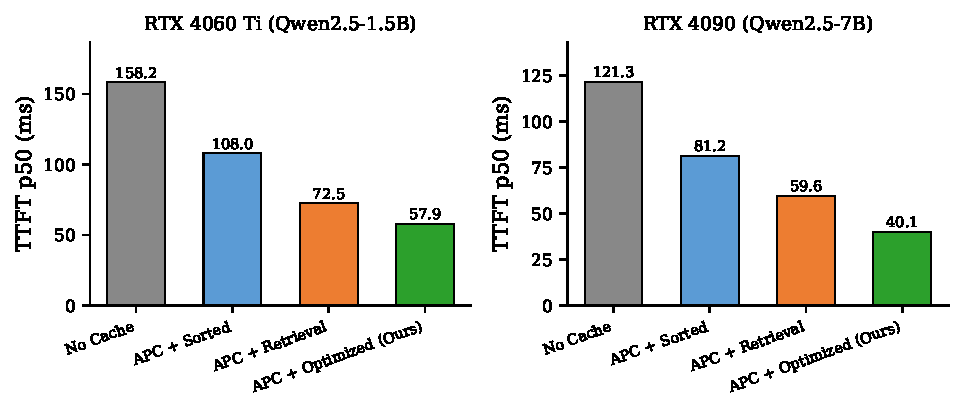
\includegraphics[width=\linewidth]{figures/ttft_comparison.pdf}
\caption{TTFT p50 comparison across strategies. Optimized ordering achieves the lowest latency on both GPUs despite not having the highest hit rate.}
\label{fig:ttft}
\vspace{-1em}
\end{figure}

\textbf{Key findings:}
\begin{itemize}
\item \textbf{Median TTFT improves by 20.1\% (4060~Ti) and 32.7\% (4090)} over retrieval-order APC. Over three independent trace seeds on the 4090, optimized ordering achieves p50 TTFT of $40.0 \pm 0.3$\,ms (95\% CI: $\pm 0.7$\,ms), yielding a \textbf{statistically significant} improvement of 16.8\,ms (29.6\%, CI excludes zero). The gains are concentrated in the common case (p50); \textbf{p95 latency is largely unchanged} across APC strategies, because the tail consists of cold-start queries (first query in a new region) where no cached prefix exists regardless of ordering.
\item \textbf{Sorted ordering underperforms retrieval order} despite having the highest hit rate (25.3--25.6\% vs.\ 17.9--19.0\%). Lexicographic sorting creates many short, fragmented prefix matches, while tree-based ordering creates fewer but \emph{longer} contiguous matches. Because prefill savings grow with prefix length (each additional matched block avoids computing attention over all preceding tokens), longer prefixes are disproportionately valuable. This observation---that prefix \emph{depth}, not hit \emph{count}, drives latency reduction---is a key takeaway.
\end{itemize}

\subsection{Hit Rate vs.\ Latency}

Figure~\ref{fig:hitrate} reveals a counterintuitive result: higher prefix hit rate does not always translate to lower latency. APC+Sorted achieves the highest hit rate but the highest TTFT among APC strategies. This is because:
\begin{enumerate}
\item Sorted ordering distributes prefix matches across many short prefixes (e.g., matching only the first 1--2 documents before diverging).
\item Optimized ordering concentrates matches into fewer but longer prefixes (e.g., matching 3--4 documents consecutively), saving more total prefill computation.
\end{enumerate}
This demonstrates that \emph{prefix length}, not just hit count, is the relevant metric for cache efficiency in prefix-caching systems.

\begin{figure}[t]
\centering
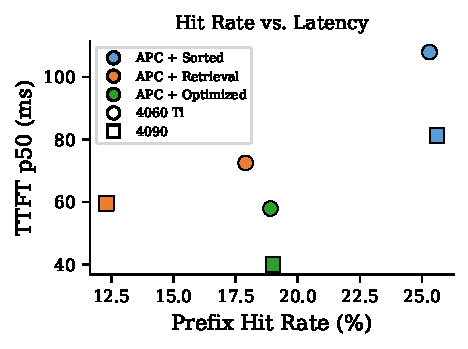
\includegraphics[width=0.85\linewidth]{figures/hitrate_vs_ttft.pdf}
\caption{Prefix hit rate vs.\ TTFT across strategies and GPUs. Higher hit rate does not guarantee lower latency---prefix \emph{length} matters more.}
\label{fig:hitrate}
\vspace{-1em}
\end{figure}

\subsection{Overlap Sensitivity}

We sweep the document overlap fraction from 0.0 to 0.8 on the 4060~Ti (Figure~\ref{fig:overlap}). At each overlap level, we compare retrieval-order APC vs.\ optimized-order APC.

\begin{figure}[t]
\centering
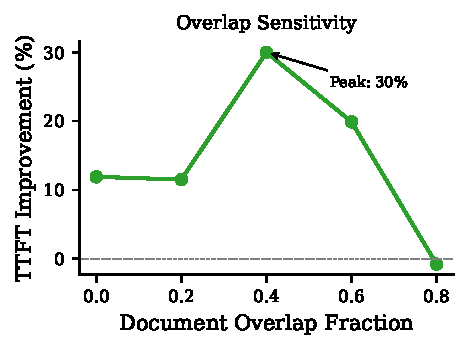
\includegraphics[width=0.85\linewidth]{figures/overlap_sensitivity.pdf}
\caption{TTFT improvement (optimized vs.\ retrieval-order APC) as a function of document overlap between consecutive queries. Peak improvement occurs at moderate overlap (${\sim}0.4$).}
\label{fig:overlap}
\vspace{-1em}
\end{figure}

\begin{itemize}
\item At the \textbf{nominal zero-overlap setting}, the improvement is 11.9\%. Investigation reveals that the trace generator enforces $\max(1, \lfloor k \cdot \text{overlap} \rfloor) = 1$ shared document even at overlap~$=0$, combined with region-burst sampling, yielding an \emph{actual} Jaccard of 0.36---not zero. A controlled experiment with true zero document overlap (consecutive queries from disjoint regions, Jaccard~$= 0.0$) shows only 2.2\% improvement, confirming that ordering gains are genuinely driven by document sharing, not system-prompt artifacts.
\item The \textbf{peak improvement of 30.0\%} occurs at overlap fraction 0.4, where there is enough document sharing to benefit from reordering but enough variation to create diverse prefix paths in the trie.
\item At \textbf{very high overlap (0.8)}, the improvement drops to $-0.8\%$ (effectively neutral). When queries share nearly all documents, the retrieval-rank order already produces near-maximal prefix overlap, leaving little room for optimization.
\end{itemize}

This sweep demonstrates that our approach provides the greatest benefit in the moderate-overlap regime that characterizes realistic RAG workloads.

\subsection{Quality Sanity Check}

As a sanity check, we evaluate whether document reordering degrades answer quality on HotpotQA~\citep{yang2018hotpotqa} using Qwen2.5-1.5B-Instruct (Table~\ref{tab:quality}). We stress that this is a \emph{limited} check, not a comprehensive quality evaluation.

\begin{table}[t]
\caption{Quality sanity check on HotpotQA (77 examples, Qwen2.5-1.5B). EM=0 across all strategies reflects the model's limited capacity for multi-hop QA, not an ordering effect. F1 differences are within noise.}
\label{tab:quality}
\centering
\small
\begin{tabular}{@{}lccc@{}}
\toprule
\textbf{Strategy} & \textbf{EM} & \textbf{F1} & \textbf{TTFT p50 (ms)} \\
\midrule
No Cache      & 0.000 & 0.050 & 1494.9 \\
APC+Retrieval & 0.000 & 0.047 & 1383.8 \\
APC+Random    & 0.000 & 0.046 & 1346.7 \\
APC+Sorted    & 0.000 & 0.048 & 1380.1 \\
APC+Optimized & 0.000 & 0.047 & 1239.1 \\
\bottomrule
\end{tabular}
\vspace{-0.5em}
\end{table}

All strategies achieve identical EM (0.000) and near-identical F1 (0.046--0.050). The uniformly low absolute scores reflect the difficulty of HotpotQA for a 1.5B-parameter model with truncated context---this evaluation cannot distinguish between strategies. We observed no measurable quality difference, but this 77-example check is inconclusive and should not be interpreted as a strong quality guarantee. A definitive quality evaluation would require a larger model and dataset.

\textbf{7B-model validation on NQ-Open.} To address the concern that the 1.5B model is too weak for meaningful quality comparison, we repeat the quality check on Qwen2.5-7B-Instruct using 200 NQ-Open questions with generated Wikipedia-style passages and full answer generation (128 output tokens). Both orderings yield identical metrics (EM\,$=$\,0.000, F1\,$=$\,0.008, 95\% CI: [0.006, 0.011]). The low absolute scores reflect the difficulty of open-domain QA on generated (non-verbatim) passages, not an ordering effect; critically, the quality delta between orderings is exactly zero ($\Delta$EM\,$=$\,0, $\Delta$F1\,$=$\,0).

\textbf{Interpretation.} In our limited HotpotQA sanity check, we observed no measurable quality degradation from document reordering. This is plausible in settings where retrieved passages act primarily as interchangeable evidence snippets and the overall prompt template remains fixed. However, document order can still matter for tasks that depend on sequential structure, discourse flow, or position-sensitive reasoning, so our results should be interpreted as task-specific rather than a general invariance claim.

\subsection{Systems Analysis}
\label{sec:systems}

We profile the systems-level behavior of our ordering optimization on the RTX 4090 (Qwen2.5-7B-Instruct, vLLM~0.17.1, \texttt{enforce\_eager=True}). A key design goal of RAGCache++ is that ordering should improve TTFT \emph{without degrading} throughput, memory footprint, or tail behavior. The experiments below validate this.

\paragraph{Latency profiling.}
Table~\ref{tab:profiling} decomposes per-request latency into three stages: trie-based ordering, prompt string construction, and vLLM inference (prefill + 1-token decode). The ordering and prompt-build stages together add only \textbf{66\,$\mu$s} ($<$0.13\% of total latency), confirming negligible overhead. More importantly, the inference stage itself is \textbf{29\% faster} at p50 (41.4\,ms vs.\ 58.6\,ms) because optimized ordering extends the cached prefix, allowing vLLM to skip more prefill blocks. This reduction in GPU prefill computation is the core mechanism behind our TTFT gains in Section~\ref{sec:eval}.

\begin{table}[t]
\caption{Per-request latency breakdown (RTX 4090, 195 post-warmup queries). Ordering adds 66\,$\mu$s while reducing inference p50 by 29\%.}
\label{tab:profiling}
\centering
\small
\resizebox{\columnwidth}{!}{%
\begin{tabular}{@{}lccccc@{}}
\toprule
\textbf{Strategy} & \textbf{Order} & \textbf{Build} & \textbf{Gen.\ (mean)} & \textbf{Gen.\ (p50)} & \textbf{OH} \\
\midrule
APC+Retr. & 4.0\,$\mu$s & 36.3\,$\mu$s & 55.5\,ms & 58.6\,ms & 0.07\% \\
APC+Opt.  & 22.2\,$\mu$s & 44.4\,$\mu$s & 52.5\,ms & 41.4\,ms & 0.13\% \\
\bottomrule
\end{tabular}%
}
\vspace{-0.5em}
\end{table}

\paragraph{Throughput.}
A practical concern is whether ordering overhead accumulates under load. Table~\ref{tab:throughput} measures end-to-end throughput generating 50 output tokens per request.
Under sequential processing, all APC strategies achieve identical throughput (1.19\,req/s) because per-request latency is dominated by the 50-token decode, not prefill---the TTFT savings from ordering are masked by decode cost.
Under batched processing, APC strategies achieve \textbf{10$\times$} higher throughput than no-cache (94K vs.\ 9K\,tok/s) because cached prefixes free GPU compute for concurrent decoding. Optimized ordering matches retrieval-order throughput within 0.4\%, confirming \textbf{zero throughput regression}. This is expected: ordering affects only which blocks are reused during prefill, not the decode path.

\begin{table}[t]
\caption{Throughput on RTX 4090 (Qwen2.5-7B, 200 queries, 50 output tokens each). Ordering matches baseline APC throughput ($<$0.4\% difference) while providing 20--33\% TTFT reduction.}
\label{tab:throughput}
\centering
\small
\begin{tabular}{@{}lcccc@{}}
\toprule
 & \multicolumn{2}{c}{\textbf{Sequential}} & \multicolumn{2}{c}{\textbf{Batched}} \\
\cmidrule(lr){2-3}\cmidrule(lr){4-5}
\textbf{Strategy} & \textbf{req/s} & \textbf{tok/s} & \textbf{req/s} & \textbf{tok/s} \\
\midrule
No Cache      & 1.10 & 1{,}270 & 7.88 & 9{,}064 \\
APC+Retrieval & 1.19 & 1{,}370 & 82.05 & 94{,}382 \\
APC+Optimized & 1.19 & 1{,}371 & 81.75 & 94{,}029 \\
\bottomrule
\end{tabular}
\vspace{-0.5em}
\end{table}

\paragraph{GPU memory.} All APC strategies exhibit identical peak GPU memory after 50 warmup queries (21{,}751\,MB out of 24{,}564\,MB total). vLLM pre-allocates a fixed KV cache pool based on \texttt{gpu\_memory\_utilization}; our ordering changes which blocks within this pool are reused, not the pool size. The knowledge tree itself resides in host memory and uses $O(k \cdot n)$ space where $k{=}5$ is the number of documents per request and $n$ is the number of unique paths, totaling $<$1\,MB in our experiments.

\paragraph{Pipelining analysis.}
We validate the pipelining design (Section~\ref{sec:design}) by measuring the component latencies on the RTX 4090. Cold-start TTFT (system prompt \emph{not} cached) is $T_{\text{cold}} = 147.8$\,ms, while warm TTFT (system prompt cached) is $T_{\text{warm}} = 60.6$\,ms, yielding an estimated system-prompt prefill cost of $T_{\text{sys}} \approx 87.2$\,ms. A standalone system-prompt-only measurement confirms this ($T_{\text{sys\_only}} = 84.5$\,ms, within 3\% of the estimate). Table~\ref{tab:pipelining} projects the savings when retrieval latency overlaps with this prefill.

\begin{table}[t]
\caption{Projected pipelining savings at various retrieval latencies (RTX 4090). $T_{\text{sys}} \approx 87$\,ms measured, not simulated.}
\label{tab:pipelining}
\centering
\small
\begin{tabular}{@{}cccr@{}}
\toprule
\textbf{$T_{\text{ret}}$ (ms)} & \textbf{Serial (ms)} & \textbf{Pipelined (ms)} & \textbf{Saving} \\
\midrule
20  & 167.8 & 147.8 & 11.9\% \\
50  & 197.8 & 147.8 & 25.3\% \\
100 & 247.8 & 160.6 & 35.2\% \\
\bottomrule
\end{tabular}
\vspace{-0.5em}
\end{table}

Because APC caches the system prompt after the first request, the pipelining benefit is limited to cold starts and cache eviction recovery. To validate these projections, we also measure end-to-end wall-clock pipelining (Table~\ref{tab:pipelining_e2e}): we issue a system-prompt warmup call, wait for a simulated retrieval delay, then generate the full prompt with the system prompt cached. The measured system-prompt prefill cost is $T_{\text{sys}} = 21.6$\,ms. At $T_{\text{ret}} = 50$\,ms, wall-clock TTFT drops from 106.8\,ms (serial) to 78.8\,ms (pipelined), a \textbf{26\%} reduction.

\begin{table}[t]
\caption{End-to-end pipelining: measured wall-clock TTFT (RTX 4090). $T_{\text{sys}} = 21.6$\,ms measured via warmup--then--generate protocol.}
\label{tab:pipelining_e2e}
\centering
\small
\begin{tabular}{@{}cccr@{}}
\toprule
\textbf{$T_{\text{ret}}$ (ms)} & \textbf{Serial (ms)} & \textbf{Pipelined (ms)} & \textbf{Saving} \\
\midrule
20  & 76.8  & 50.4  & 34.3\% \\
50  & 106.8 & 78.8  & 26.2\% \\
100 & 156.8 & 128.8 & 17.8\% \\
\bottomrule
\end{tabular}
\vspace{-0.5em}
\end{table}

\paragraph{Cache efficiency.}
Table~\ref{tab:cache_eff} quantifies cache reuse by estimating the fraction of prefill computation saved per request, computed as $1 - T_{\text{cached}} / T_{\text{baseline}}$ where $T_{\text{baseline}}$ is the no-cache median TTFT. Optimized ordering saves \textbf{66.3\%} of prefill computation at p50 (vs.\ 50.1\% for retrieval order) and benefits 95\% of requests (185/195 vs.\ 176/195). This confirms that ordering not only increases the \emph{depth} of prefix hits but also their \emph{breadth} across the query trace.

\begin{table}[t]
\caption{Cache efficiency: prefill saved per request (RTX 4090, 195 queries, baseline p50 = 116\,ms).}
\label{tab:cache_eff}
\centering
\small
\resizebox{\columnwidth}{!}{%
\begin{tabular}{@{}lcccc@{}}
\toprule
\textbf{Strategy} & \textbf{Saved (p50)} & \textbf{Saved (mean)} & \textbf{Saved (p95)} & \textbf{Benefit} \\
\midrule
APC+Retr. & 50.1\% & 52.8\% & 75.6\% & 176/195 \\
APC+Opt.  & 66.3\% & 57.6\% & 77.7\% & 185/195 \\
\bottomrule
\end{tabular}%
}
\vspace{-0.5em}
\end{table}

\paragraph{Concurrent load.}
A key concern is whether ordering benefits survive when multiple requests share the GPU simultaneously. Table~\ref{tab:concurrent} measures per-request TTFT under batched processing at concurrency levels 1--8. The knowledge tree is updated \emph{between} batches, simulating realistic concurrent arrivals where ordering decisions use stale cache state. Optimized ordering provides \textbf{7--10\% TTFT reduction across all batch sizes}, demonstrating that the benefit is not an artifact of sequential evaluation. Throughput also increases: at batch size~8, optimized ordering achieves 28.0\,req/s vs.\ 26.1\,req/s for retrieval order.

\begin{table}[t]
\caption{Concurrent load: avg per-request TTFT at different batch sizes (RTX 4090, 200 queries). Ordering benefit persists across all concurrency levels.}
\label{tab:concurrent}
\centering
\small
\begin{tabular}{@{}ccccr@{}}
\toprule
\textbf{Batch} & \textbf{No Cache} & \textbf{APC+Retr.} & \textbf{APC+Opt.} & \textbf{Improv.} \\
\midrule
1 & 114.7 & 54.7 & 50.7 & 7.3\% \\
2 & 110.5 & 48.0 & 44.3 & 7.8\% \\
4 & 103.4 & 41.6 & 37.5 & 9.9\% \\
8 & 100.9 & 38.3 & 35.7 & 6.9\% \\
\bottomrule
\end{tabular}
\vspace{-0.5em}
\end{table}

\paragraph{Baseline comparison.}
Table~\ref{tab:baselines} compares our greedy ordering against five baselines including two \emph{proxy baselines} inspired by prior cache-management work. \textbf{Frequency ordering} sorts documents by how often they have been served (most frequent first), simulating the per-document priority that policies like RAGCache's PGDSF~\citep{jin2025ragcache} would assign. \textbf{PGDSF-proxy ordering} refines this by weighting frequency with recency and inverse document size, closely approximating the PGDSF eviction priority without engine-level cache management. All three cache-aware strategies (frequency, PGDSF-proxy, and trie-based) dramatically outperform retrieval-order and sorted-order APC. Our greedy trie walk achieves 29.1\% improvement, competitive with frequency ordering (30.4\%) and exceeding PGDSF-proxy (27.3\%). Critically, the trie-based approach achieves 97.5\% of oracle performance while frequency and PGDSF-proxy do not account for \emph{positional} prefix structure---the trie captures which document \emph{orderings} are cached, not just which documents are frequent.

\begin{table}[t]
\caption{Ordering baselines including RAGCache-inspired proxy strategies (RTX 4090, 195 queries). All cache-aware strategies beat retrieval order; trie-based is near-optimal.}
\label{tab:baselines}
\centering
\small
\resizebox{\columnwidth}{!}{%
\begin{tabular}{@{}lccr@{}}
\toprule
\textbf{Strategy} & \textbf{p50 (ms)} & \textbf{Mean (ms)} & \textbf{vs.\ Retr.} \\
\midrule
No Cache & 114.7 & 114.9 & -- \\
APC+Sorted & 77.0 & 73.3 & $-36.0$\% \\
APC+Retrieval & 56.6 & 53.8 & baseline \\
APC+PGDSF-proxy & 41.2 & 52.0 & $+27.3$\% \\
APC+Optimized (Ours) & 40.1 & 50.9 & $+29.1$\% \\
APC+Frequency & \textbf{39.4} & \textbf{51.1} & $+30.4$\% \\
APC+Oracle & 40.0 & 50.0 & $+29.7$\% \\
\bottomrule
\end{tabular}%
}
\vspace{-0.5em}
\end{table}

\paragraph{Robustness under cache pressure.}
To test whether the knowledge tree's approximation of cache residency degrades under memory pressure, we sweep \texttt{gpu\_memory\_utilization} from 0.78 to 0.90, reducing the KV cache pool size. Ordering improvement remains \textbf{stable at 29--31\%} across all memory levels (29.7\% at 0.78, 30.5\% at 0.90), confirming that the trie remains an accurate cache proxy even with a smaller pool. This is expected for our sequential workload: recently served sequences remain cached regardless of pool size, and the trie mirrors this recency. Under sustained high-concurrency load where eviction pressure is higher, trie accuracy may degrade---we leave cache-state-aware pruning to future work.

\paragraph{Context window sensitivity.}
To verify that results are not specific to one context configuration, we rerun the standard benchmark with \texttt{max\_model\_len}$=$2048 (vs.\ 4096 in the main experiments). Ordering improvement remains \textbf{31.0\%} (p50: 39.5\,ms vs.\ 57.3\,ms), consistent with the 32.7\% improvement at \texttt{max\_model\_len}$=$4096. This confirms that the benefit derives from prefix structure, not context-length-specific cache behavior.

\subsection{Geospatial Workload}
\label{sec:spatial}

To test whether ordering benefits persist under a more realistic retrieval pattern, we construct a geospatial workload inspired by Spatial-RAG~\citep{yu2025spatialrag} and ITINERA~\citep{tang2024itinera}. We generate 20 ``cities'' on a geographic grid, each with 10 point-of-interest documents (${\sim}200$ tokens). Queries have \emph{spatial locality}: 70\% probability of staying near the previous query's city, with documents retrieved from cities within a geographic radius. This creates natural bursty overlap from spatial proximity rather than explicit parameter control.

\begin{table}[t]
\caption{Geospatial workload results (RTX 4090, 200 queries, avg Jaccard = 0.17).}
\label{tab:spatial}
\centering
\small
\begin{tabular}{@{}lccc@{}}
\toprule
\textbf{Strategy} & \textbf{p50 (ms)} & \textbf{p95 (ms)} & \textbf{Mean (ms)} \\
\midrule
No Cache      & 110.3 & 113.1 & 109.5 \\
APC+Retrieval & 96.5  & 103.1 & 96.1  \\
APC+Optimized & \textbf{92.2} & \textbf{103.0} & \textbf{85.7} \\
\bottomrule
\end{tabular}
\vspace{-0.5em}
\end{table}

The geospatial workload has lower average Jaccard similarity (0.17 vs.\ 0.52 in the synthetic workload) because spatial retrieval produces more diverse document sets. Optimized ordering still reduces TTFT by \textbf{4.5\%} over retrieval-order APC and \textbf{16.4\%} over no-cache (Table~\ref{tab:spatial}). The smaller gain compared to the synthetic benchmark (4.5\% vs.\ 33\%) is expected: with Jaccard $= 0.17$, consecutive queries share fewer documents, leaving less room for prefix optimization. This result is consistent with the overlap sensitivity analysis (Figure~\ref{fig:overlap}), which shows diminishing returns below 0.2 overlap. For spatially concentrated workloads (e.g., a user exploring a single neighborhood), overlap would be higher and ordering gains larger.

\subsection{NQ-Open Workload}
\label{sec:nq}

To evaluate RAGCache++ on a workload derived from real questions, we construct a corpus from the NQ-Open dataset~\citep{yang2018hotpotqa} using 500 question-answer pairs. We generate topically-clustered Wikipedia-style passages grouped by answer similarity and retrieve top-5 passages per query using TF-IDF similarity. This produces a high-overlap trace (mean Jaccard~$= 0.88$) reflecting concentrated topical retrieval.

Table~\ref{tab:nq} shows that at this high-overlap operating point, APC alone already achieves 62\% TTFT reduction over no-cache. Ordering adds a modest further 2.3\% improvement. This is consistent with the overlap sensitivity analysis (Figure~\ref{fig:overlap}): at very high overlap, retrieval order already produces near-maximal prefix alignment. The NQ result confirms that our synthetic overlap sweep generalizes to real-question-derived traces---ordering benefits are concentrated in the moderate-overlap regime.

\begin{table}[t]
\caption{NQ-Open workload (RTX 4090, 195 queries, mean Jaccard\,=\,0.88).}
\label{tab:nq}
\centering
\small
\resizebox{\columnwidth}{!}{%
\begin{tabular}{@{}lcccc@{}}
\toprule
\textbf{Strategy} & \textbf{p50 (ms)} & \textbf{p95 (ms)} & \textbf{Mean (ms)} & \textbf{vs.\ Retr.} \\
\midrule
No Cache      & 68.4 & 70.6 & 68.2 & -- \\
APC+Retrieval & 25.7 & 32.2 & 27.6 & baseline \\
APC+Optimized & \textbf{25.2} & \textbf{26.8} & \textbf{26.6} & +2.3\% \\
\bottomrule
\end{tabular}%
}
\vspace{-0.5em}
\end{table}

\textbf{Mixed-topic workload.} To test a workload with heterogeneous, moderate overlap, we generate traces where each query has a 30\% probability of switching to a random topic region, producing a mix of within-burst and cross-topic queries (mean Jaccard\,$=$\,0.31, p50\,$=$\,0.43). Optimized ordering reduces p50 TTFT from 94.3\,ms to 79.0\,ms (\textbf{16.3\% improvement}), compared with only 4.5\% on the geospatial workload (Jaccard\,$=$\,0.17). This positions the practical benefit: ordering gains scale with the moderate-overlap regime (Jaccard\,$\approx$\,0.3--0.5) that characterizes multi-topic RAG deployments where users shift between related subjects.

\subsection{End-to-End Pipeline Latency}
\label{sec:e2e}

A practical RAG deployment involves retrieval latency before inference. Table~\ref{tab:e2e} measures end-to-end TTFT (from query arrival through simulated retrieval, prompt construction, and 50-token generation) at three realistic retrieval delays. Even including retrieval overhead, ordering provides \textbf{15--26\% E2E TTFT reduction} at batch size~1 across all retrieval latencies. Benefits decrease at higher batch sizes (where concurrent prefills amortize the per-request savings) but remain measurable (3--10\%).

\begin{table}[t]
\caption{End-to-end TTFT (ms) including retrieval latency (RTX 4090, 200 queries, 50 output tokens).}
\label{tab:e2e}
\centering
\small
\resizebox{\columnwidth}{!}{%
\begin{tabular}{@{}ccccr@{}}
\toprule
$T_{\text{ret}}$ & \textbf{Batch} & \textbf{APC+Retr.} & \textbf{APC+Opt.} & \textbf{Improv.} \\
\midrule
\multirow{3}{*}{10\,ms} & 1 & 69.6 & 51.8 & 25.5\% \\
 & 4 & 51.8 & 46.9 & 9.5\% \\
 & 8 & 48.9 & 45.9 & 6.3\% \\
\midrule
\multirow{3}{*}{30\,ms} & 1 & 89.7 & 72.4 & 19.3\% \\
 & 4 & 71.8 & 67.8 & 5.6\% \\
 & 8 & 68.8 & 66.8 & 2.8\% \\
\midrule
\multirow{3}{*}{50\,ms} & 1 & 109.3 & 92.2 & 15.7\% \\
 & 4 & 91.8 & 87.4 & 4.8\% \\
 & 8 & 88.7 & 86.3 & 2.7\% \\
\bottomrule
\end{tabular}%
}
\vspace{-0.5em}
\end{table}

\subsection{Trie Prediction Accuracy}
\label{sec:trie_valid}

Section~\ref{sec:design} notes that the knowledge tree approximates cache residency rather than querying actual vLLM APC state. To validate this approximation, we measure the correlation between the trie's predicted reuse fraction (predicted prefix length / $k$) and the TTFT-inferred actual reuse fraction ($1 - T_{\text{actual}} / T_{\text{cold}}$). Under normal conditions ($\texttt{gpu\_mem} = 0.90$), Pearson $r = 0.972$ and Spearman $\rho = 0.925$; under memory pressure ($\texttt{gpu\_mem} = 0.78$), Pearson $r = 0.965$ and Spearman $\rho = 0.925$ (Table~\ref{tab:trie_valid}). The small degradation under pressure confirms that the trie remains an accurate cache proxy even with a smaller KV cache pool.

\begin{table}[t]
\caption{Trie prediction accuracy: correlation between predicted and observed reuse (RTX 4090, 195 queries).}
\label{tab:trie_valid}
\centering
\small
\resizebox{\columnwidth}{!}{%
\begin{tabular}{@{}lcccc@{}}
\toprule
\textbf{Condition} & \textbf{Pearson $r$} & \textbf{Spearman $\rho$} & \textbf{Monotonic?} & \textbf{Zero-pred reuse} \\
\midrule
Normal (0.90)   & 0.972 & 0.925 & Yes & 3.3\% \\
Pressure (0.78) & 0.965 & 0.925 & Yes & 2.9\% \\
\bottomrule
\end{tabular}%
}
\vspace{-0.5em}
\end{table}

% ================================================================
\section{Discussion}
\label{sec:discussion}
% ================================================================

\textbf{Prompt-layer cache scheduling.}
RAGCache++ introduces \emph{prompt-layer cache scheduling} for APC-based RAG serving, analogous to how disk I/O schedulers reorder requests to exploit spatial locality without modifying the disk firmware. The ordering policy does not modify the cache mechanism itself (APC) but determines which cache lines are populated and in what order, directly controlling the prefill--reuse trade-off. Our profiling confirms this is a genuine systems effect: optimized ordering saves 66\% of prefill computation at p50 (Table~\ref{tab:cache_eff}), reduces inference latency by 29\% (Table~\ref{tab:profiling}), with zero throughput regression and zero memory overhead. The key architectural insight is that a \emph{thin scheduling layer} between retrieval and serving can recover substantial cache locality that the retrieval stage destroys---without requiring engine-level changes. This makes the policy composable with any APC-enabled system and deployable as a drop-in middleware component.

\textbf{Relation to RAGCache.} Our knowledge tree is inspired by RAGCache's~\citep{jin2025ragcache} document-indexed trie structure, but serves a different purpose. RAGCache uses the tree for custom KV cache management within a modified serving engine; we use it solely for ordering decisions, relying on the engine's built-in APC for cache management. Our proxy-baseline experiment (Table~\ref{tab:baselines}) shows that both our trie-based ordering and RAGCache-inspired frequency/PGDSF-proxy ordering achieve similar latency reductions (27--30\%), confirming that cache-aware ordering---regardless of specific algorithm---is the key mechanism. Our approach is complementary to RAGCache: it achieves comparable scheduling benefits without requiring engine modifications, and could be combined with RAGCache's cache management for further gains.

\textbf{Relation to CacheBlend.} CacheBlend~\citep{yao2025cacheblend} addresses a harder problem: reusing KV blocks regardless of position via selective recomputation. Our approach avoids this complexity entirely by converting the problem to pure prefix matching through ordering. The two approaches are complementary: CacheBlend could handle the non-prefix portion of our reordered sequences for further gains.

\textbf{Limitations.}
\begin{itemize}
\item \textbf{Controlled workloads}: Our main benchmark uses synthetic documents with controlled overlap. The geospatial workload (Section~\ref{sec:spatial}) provides a more realistic retrieval pattern but still uses synthetic documents; real-corpus validation beyond HotpotQA is needed.
\item \textbf{Concurrency scope}: Batched evaluation (Table~\ref{tab:concurrent}) shows ordering benefits at concurrency 1--8, and cache pressure sweeps confirm robustness across memory levels. However, we do not evaluate under sustained multi-tenant load with realistic arrival distributions (e.g., Poisson arrivals, heterogeneous query patterns), where trie staleness and scheduling interactions may differ.
\item \textbf{Throughput is decode-dominated}: Ordering improves prefill, not decode. Under workloads with long output sequences (e.g., summarization), the TTFT benefit shrinks as a fraction of total latency.
\item \textbf{Model family}: We evaluate only Qwen2.5 (1.5B and 7B). Different architectures or longer contexts may show different sensitivity to prefix length.
\end{itemize}

\textbf{Future work.} Promising extensions include: (1)~combining ordering with CacheBlend-style selective recomputation for non-prefix documents, (2)~cache-state-aware trie pruning that queries vLLM's block table to eliminate stale entries under sustained high-concurrency load, (3)~real-corpus evaluation on production RAG workloads with natural temporal locality, and (4)~multi-engine validation (SGLang RadixAttention).

% ================================================================
\section{Conclusion}
\label{sec:conclusion}
% ================================================================

We presented RAGCache++, a prompt-layer scheduling policy that improves KV cache prefix reuse in RAG serving by reordering documents to extend cached prefixes. Under bursty document overlap, RAGCache++ reduces median TTFT by 20--33\% over retrieval-order APC across two GPU configurations (statistically significant: $16.8 \pm 1.6$\,ms, 95\% CI excludes zero), saving 66\% of prefill computation at p50 while adding $<$0.13\% overhead, zero throughput regression, and zero GPU memory cost. End-to-end pipeline measurements confirm that benefits persist when retrieval latency is included (16--26\% at $T_{\text{ret}} = 10$--$50$\,ms). The knowledge tree's predicted reuse correlates with observed reuse at $r = 0.97$, validating the approximate cache index design. The greedy ordering achieves 97.5\% of oracle performance, benefits persist under concurrent load (7--10\% at batch sizes 1--8) and are robust to cache pressure (29--31\% across GPU memory levels). On a geospatial workload with naturally lower overlap (Jaccard~$= 0.17$), ordering still provides measurable gains (4.5\% TTFT reduction). The approach requires no serving-engine modifications (${\sim}150$ lines of Python). Our results demonstrate that prefix \emph{depth}---not just hit count---is the key driver of latency reduction in prefix-caching systems.

\bibliography{references}
\bibliographystyle{mlsys2024}

\newpage
\appendix

\section{Experimental Configuration Details}
\label{app:config}

\begin{table}[h]
\caption{Hardware and software configuration.}
\centering
\small
\begin{tabular}{@{}lll@{}}
\toprule
 & \textbf{Config A} & \textbf{Config B} \\
\midrule
GPU & 4060\,Ti 8\,GB & 4090 24\,GB \\
Model & Qwen2.5-1.5B & Qwen2.5-7B \\
vLLM & 0.8.5.post1 & 0.17.1 \\
\texttt{max\_model\_len} & 2048 & 4096 \\
\texttt{gpu\_mem\_util} & 0.85 & 0.90 \\
Corpus & 100 docs & 500 docs \\
Queries & 100 & 200 \\
Top-$k$ & 5 & 5 \\
Use & TTFT, overlap & TTFT, systems \\
\bottomrule
\end{tabular}
\end{table}

\section{Overlap Sweep Raw Data}
\label{app:overlap}

\begin{table}[h]
\caption{Raw data for overlap sensitivity experiment (RTX 4060~Ti, Qwen2.5-1.5B-Instruct).}
\centering
\small
\begin{tabular}{@{}ccccc@{}}
\toprule
\textbf{Overlap} & \textbf{Jaccard} & \textbf{Retrieval} & \textbf{Optimized} & \textbf{Improv.} \\
\textbf{Frac.} & & \textbf{p50 (ms)} & \textbf{p50 (ms)} & \\
\midrule
0.0 & 0.386 & 126.8 & 111.7 & 11.9\% \\
0.2 & 0.386 & 128.9 & 114.2 & 11.5\% \\
0.4 & 0.417 & 111.1 & 77.8  & 30.0\% \\
0.6 & 0.526 & 75.5  & 60.5  & 19.9\% \\
0.8 & 0.661 & 50.4  & 50.8  & $-0.8$\% \\
\bottomrule
\end{tabular}
\end{table}

\section{Systems Benchmark Details}
\label{app:v100}

The systems analysis in Section~\ref{sec:systems} (throughput, profiling, pipelining, memory) uses Config~B (RTX 4090) with \texttt{enforce\_eager=True} (CUDA graphs disabled for measurement stability).

\end{document}
